\subsection*{a}
The mass of the atom is given by
\begin{equation*}
    M(^{48}_{20}\text{Ca}^{28}) = Z(m_p + m_e) + (A-Z)m_n - \frac{B(A, Z)}{c^2}
    \label{eq:semi_empirical_mass_formula}
\end{equation*}
where $B$ indicates the binding energy, which in turns can be calculated via the semi-empirical formula (atomic units)
\begin{equation}
    B(A, Z)= a_v A - a_s A^{2/3} - a_c \frac{Z(Z-1)}{A^{1/3}} - a_{sym} \frac{(A - 2Z)^2}{A} + \delta (A, Z)
    \label{eq:semi_empirical_BE_formula}
\end{equation}
where 
\begin{equation*}
    \delta(A, Z) = 
    \begin{cases}
        \frac{a_P}{A^{1/2}} \qquad \text{if Z and N are even} \\
        0 \qquad \text{if A is odd} \\
        -\frac{a_P}{A^{1/2}} \qquad \text{if Z and N are odd} 
    \end{cases}
\end{equation*}
One can simply pop in the values of $A$ and $Z$ into the formula using the fitted coefficients (source Wikipedia) in units of $MeV/c^2$
\begin{equation*}
    a_v = 15.8 \qquad a_s = 18.3 \qquad a_c = 0.714 \qquad a_{sym} = 23.2 \qquad a_P = 12
\end{equation*}
and obtains $B(A, Z) = 412.84~MeV/c^2$. Hence, inserting the result into \ref{eq:semi_empirical_mass_formula} one obtains
\begin{equation*}
    M(^{48}\text{Ca}) \simeq 44670.64~MeV/c^2 \simeq 47.96~u
\end{equation*}
The result is close to the experimental value ($47.952)$. One could justify eventual differences by observing that the SEMF is 
not a complete theoretical model, but rather a fit to experimental data of a model with some theoretical fundations. As such, it is reasonable that the model
can give an overall good description of the data but cannot perfectly describe each of them: this is especially the case of lighter atoms for which
the quantum shell structures of the nucleus should be taken into account.

\subsection*{b}
One can calculate the energy to remove a neutron as the difference in energy between the atom's state with the neutron and without the neutron. The energy is the sum of
two terms, one that take accounts of the mass of the particles and it is simply the sum of all the masses. The second term, instead, is the binding energy. In the initial and final
state the mass energy contributions are the same (we are not making any particle disappear, we are just moving one away), hence the difference is only due to the binding energy contribution. One can
calculate this contribution as
\begin{equation*}
    B_{neutron} = B(A, Z) - B(A-1, Z)
\end{equation*}
and using expression \ref{eq:semi_empirical_BE_formula} with $A=44$ and $Z=20$ to calculate the two quantities one ends up with an estimation for the energy required to extract the neutron
\begin{equation*}
    \Delta E_{neutron} \approx 11.14~MeV/c^2
\end{equation*}

\subsection*{c}
One can search for the most stable atom with fixed $A$ searching for the minimum of the mass formula
\begin{equation*}
    M_A(Z) = Z(m_p + m_e) + (A-Z)m_n - B_A(Z)
\end{equation*}
Since one does not know if $Z$ is even or odd in advance, one can set the pairing term in the binding energy to $0$: this will lead to a non-integer $Z$ and 
the true minimum value will be either the closest greater or smaller integer (one has to check which of the two has minimum energy).
By direct calculation
\begin{equation*}
    0 = \frac{dM_A}{dZ} = m_p + m_e - m_n - \frac{a_c}{A^{1/3}} \left(A-2Z\right) + 4\frac{a_{symm}}{A} \left(A-2Z\right)
\end{equation*}
and rearranging terms
\begin{equation*}
    Z = \frac{m_n - (m_p + m_e) + 4a_{symm}A + a_c A^{2/3}}{2a_c A^{2/3} + 8a_{symm}} \approx 56.59 \qquad \longrightarrow \qquad Z = 56
\end{equation*}
Figures \ref{fig:even} and \ref{fig:odd} report a plot of the nuclus masses as a function of the atomic number $Z$ for fixed $A$ using the mass 
semi-empirical formula. The odd A plot contains only one parabola, while the even A plot contains two parabolas: this is becaus of the pairing term in the 
MSEF, which is either positive if $Z$ is even or negative if $Z$ is odd. In both cases, atoms which do not lie in the minimum tend to decay via $\beta$-decay towards
the most stable configuration (the minimum of the parabola) by changing neutrons into protons and vice-versa. 
\begin{figure}
    \centering
    \begin{minipage}{0.4\textwidth}
        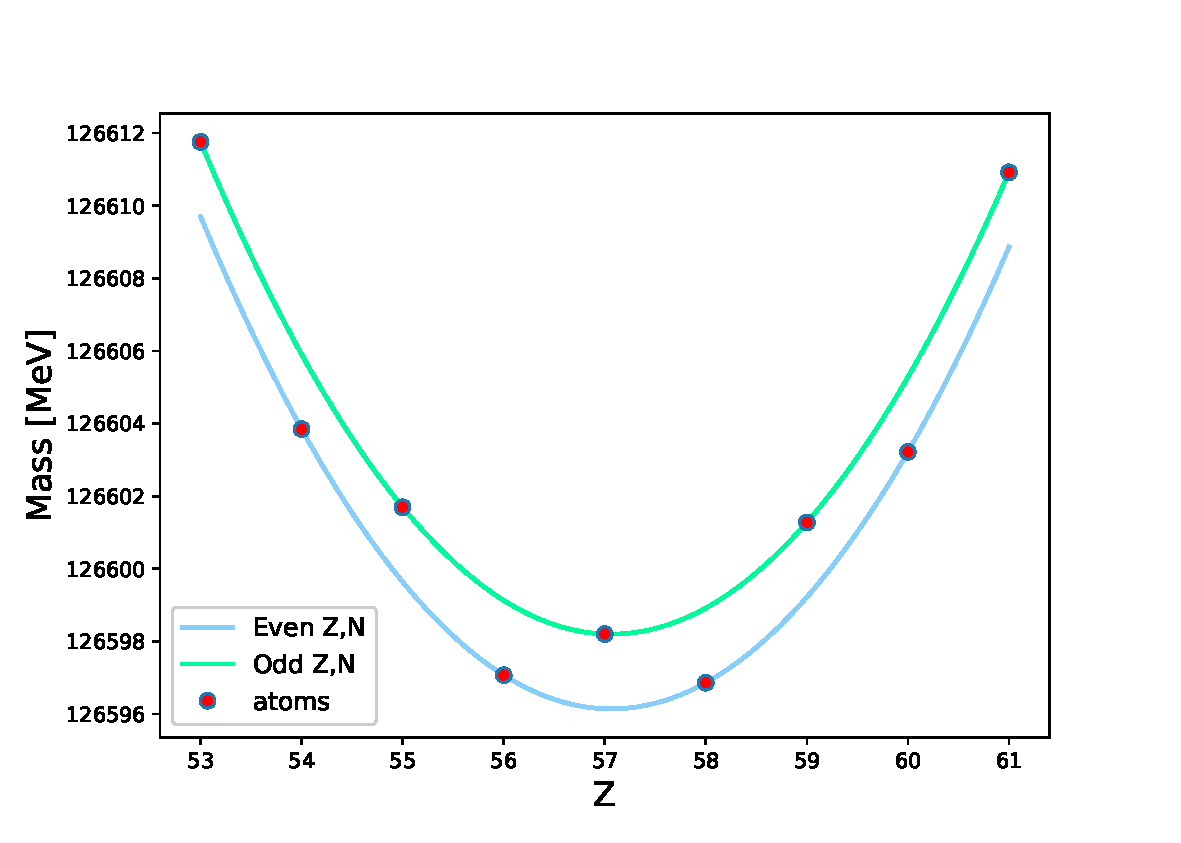
\includegraphics[scale=0.42]{ex2/evenA.eps}
        \caption{Even A}
        \label{fig:even}
    \end{minipage}
    \hspace{0.1\textwidth}
    \begin{minipage}{0.4\textwidth}
        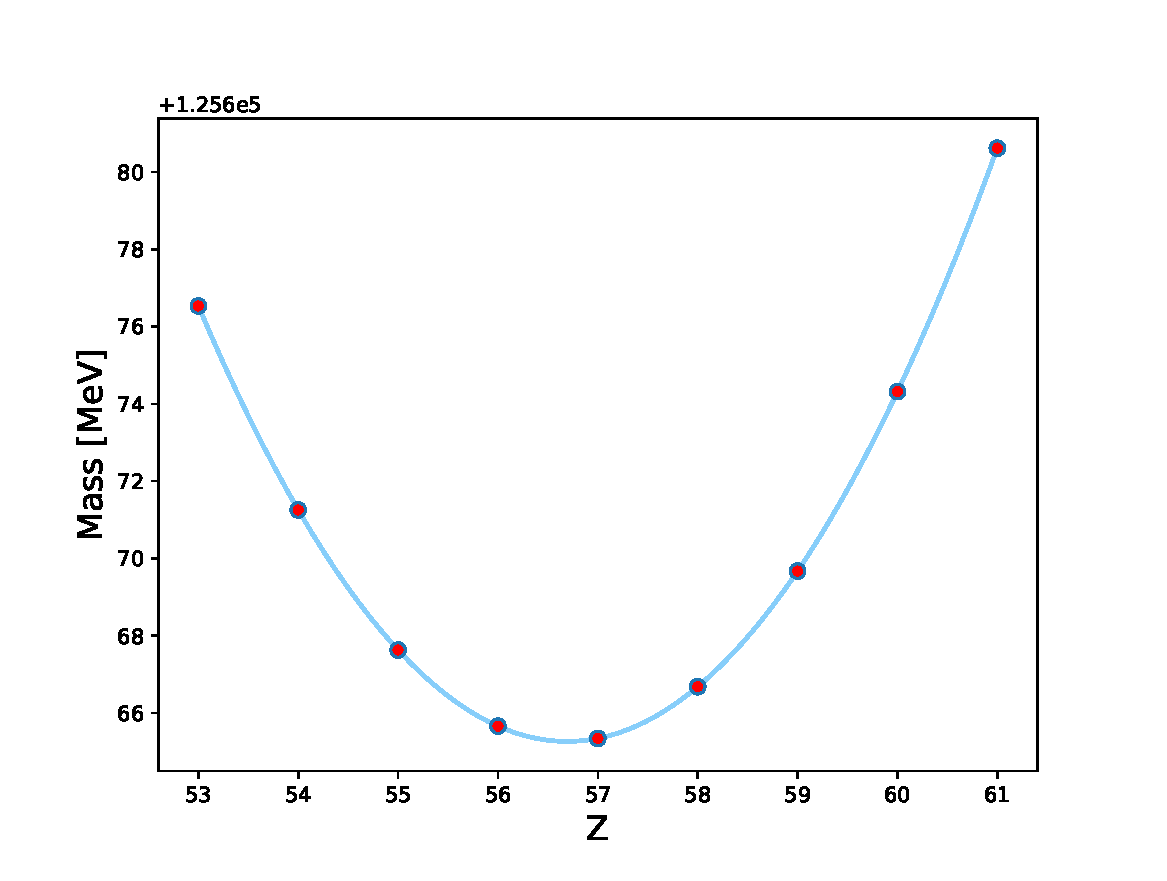
\includegraphics[scale=0.4]{ex2/oddA.eps}
        \caption{Odd A}
        \label{fig:odd}
    \end{minipage}
    
\end{figure}